% Options for packages loaded elsewhere
\PassOptionsToPackage{unicode}{hyperref}
\PassOptionsToPackage{hyphens}{url}
%
\documentclass[
]{book}
\usepackage{lmodern}
\usepackage{amssymb,amsmath}
\usepackage{ifxetex,ifluatex}
\ifnum 0\ifxetex 1\fi\ifluatex 1\fi=0 % if pdftex
  \usepackage[T1]{fontenc}
  \usepackage[utf8]{inputenc}
  \usepackage{textcomp} % provide euro and other symbols
\else % if luatex or xetex
  \usepackage{unicode-math}
  \defaultfontfeatures{Scale=MatchLowercase}
  \defaultfontfeatures[\rmfamily]{Ligatures=TeX,Scale=1}
\fi
% Use upquote if available, for straight quotes in verbatim environments
\IfFileExists{upquote.sty}{\usepackage{upquote}}{}
\IfFileExists{microtype.sty}{% use microtype if available
  \usepackage[]{microtype}
  \UseMicrotypeSet[protrusion]{basicmath} % disable protrusion for tt fonts
}{}
\makeatletter
\@ifundefined{KOMAClassName}{% if non-KOMA class
  \IfFileExists{parskip.sty}{%
    \usepackage{parskip}
  }{% else
    \setlength{\parindent}{0pt}
    \setlength{\parskip}{6pt plus 2pt minus 1pt}}
}{% if KOMA class
  \KOMAoptions{parskip=half}}
\makeatother
\usepackage{xcolor}
\IfFileExists{xurl.sty}{\usepackage{xurl}}{} % add URL line breaks if available
\IfFileExists{bookmark.sty}{\usepackage{bookmark}}{\usepackage{hyperref}}
\hypersetup{
  pdftitle={Learning LogBook Tree phenology analysis with R},
  pdfauthor={Philipp Münker},
  hidelinks,
  pdfcreator={LaTeX via pandoc}}
\urlstyle{same} % disable monospaced font for URLs
\usepackage{color}
\usepackage{fancyvrb}
\newcommand{\VerbBar}{|}
\newcommand{\VERB}{\Verb[commandchars=\\\{\}]}
\DefineVerbatimEnvironment{Highlighting}{Verbatim}{commandchars=\\\{\}}
% Add ',fontsize=\small' for more characters per line
\usepackage{framed}
\definecolor{shadecolor}{RGB}{248,248,248}
\newenvironment{Shaded}{\begin{snugshade}}{\end{snugshade}}
\newcommand{\AlertTok}[1]{\textcolor[rgb]{0.94,0.16,0.16}{#1}}
\newcommand{\AnnotationTok}[1]{\textcolor[rgb]{0.56,0.35,0.01}{\textbf{\textit{#1}}}}
\newcommand{\AttributeTok}[1]{\textcolor[rgb]{0.77,0.63,0.00}{#1}}
\newcommand{\BaseNTok}[1]{\textcolor[rgb]{0.00,0.00,0.81}{#1}}
\newcommand{\BuiltInTok}[1]{#1}
\newcommand{\CharTok}[1]{\textcolor[rgb]{0.31,0.60,0.02}{#1}}
\newcommand{\CommentTok}[1]{\textcolor[rgb]{0.56,0.35,0.01}{\textit{#1}}}
\newcommand{\CommentVarTok}[1]{\textcolor[rgb]{0.56,0.35,0.01}{\textbf{\textit{#1}}}}
\newcommand{\ConstantTok}[1]{\textcolor[rgb]{0.00,0.00,0.00}{#1}}
\newcommand{\ControlFlowTok}[1]{\textcolor[rgb]{0.13,0.29,0.53}{\textbf{#1}}}
\newcommand{\DataTypeTok}[1]{\textcolor[rgb]{0.13,0.29,0.53}{#1}}
\newcommand{\DecValTok}[1]{\textcolor[rgb]{0.00,0.00,0.81}{#1}}
\newcommand{\DocumentationTok}[1]{\textcolor[rgb]{0.56,0.35,0.01}{\textbf{\textit{#1}}}}
\newcommand{\ErrorTok}[1]{\textcolor[rgb]{0.64,0.00,0.00}{\textbf{#1}}}
\newcommand{\ExtensionTok}[1]{#1}
\newcommand{\FloatTok}[1]{\textcolor[rgb]{0.00,0.00,0.81}{#1}}
\newcommand{\FunctionTok}[1]{\textcolor[rgb]{0.00,0.00,0.00}{#1}}
\newcommand{\ImportTok}[1]{#1}
\newcommand{\InformationTok}[1]{\textcolor[rgb]{0.56,0.35,0.01}{\textbf{\textit{#1}}}}
\newcommand{\KeywordTok}[1]{\textcolor[rgb]{0.13,0.29,0.53}{\textbf{#1}}}
\newcommand{\NormalTok}[1]{#1}
\newcommand{\OperatorTok}[1]{\textcolor[rgb]{0.81,0.36,0.00}{\textbf{#1}}}
\newcommand{\OtherTok}[1]{\textcolor[rgb]{0.56,0.35,0.01}{#1}}
\newcommand{\PreprocessorTok}[1]{\textcolor[rgb]{0.56,0.35,0.01}{\textit{#1}}}
\newcommand{\RegionMarkerTok}[1]{#1}
\newcommand{\SpecialCharTok}[1]{\textcolor[rgb]{0.00,0.00,0.00}{#1}}
\newcommand{\SpecialStringTok}[1]{\textcolor[rgb]{0.31,0.60,0.02}{#1}}
\newcommand{\StringTok}[1]{\textcolor[rgb]{0.31,0.60,0.02}{#1}}
\newcommand{\VariableTok}[1]{\textcolor[rgb]{0.00,0.00,0.00}{#1}}
\newcommand{\VerbatimStringTok}[1]{\textcolor[rgb]{0.31,0.60,0.02}{#1}}
\newcommand{\WarningTok}[1]{\textcolor[rgb]{0.56,0.35,0.01}{\textbf{\textit{#1}}}}
\usepackage{longtable,booktabs}
% Correct order of tables after \paragraph or \subparagraph
\usepackage{etoolbox}
\makeatletter
\patchcmd\longtable{\par}{\if@noskipsec\mbox{}\fi\par}{}{}
\makeatother
% Allow footnotes in longtable head/foot
\IfFileExists{footnotehyper.sty}{\usepackage{footnotehyper}}{\usepackage{footnote}}
\makesavenoteenv{longtable}
\usepackage{graphicx,grffile}
\makeatletter
\def\maxwidth{\ifdim\Gin@nat@width>\linewidth\linewidth\else\Gin@nat@width\fi}
\def\maxheight{\ifdim\Gin@nat@height>\textheight\textheight\else\Gin@nat@height\fi}
\makeatother
% Scale images if necessary, so that they will not overflow the page
% margins by default, and it is still possible to overwrite the defaults
% using explicit options in \includegraphics[width, height, ...]{}
\setkeys{Gin}{width=\maxwidth,height=\maxheight,keepaspectratio}
% Set default figure placement to htbp
\makeatletter
\def\fps@figure{htbp}
\makeatother
\setlength{\emergencystretch}{3em} % prevent overfull lines
\providecommand{\tightlist}{%
  \setlength{\itemsep}{0pt}\setlength{\parskip}{0pt}}
\setcounter{secnumdepth}{5}
\usepackage{booktabs}
\usepackage{booktabs}
\usepackage{longtable}
\usepackage{array}
\usepackage{multirow}
\usepackage{wrapfig}
\usepackage{float}
\usepackage{colortbl}
\usepackage{pdflscape}
\usepackage{tabu}
\usepackage{threeparttable}
\usepackage{threeparttablex}
\usepackage[normalem]{ulem}
\usepackage{makecell}
\usepackage{xcolor}
\usepackage[]{natbib}
\bibliographystyle{plainnat}

\title{Learning LogBook Tree phenology analysis with R}
\author{Philipp Münker}
\date{2022-12-26}

\begin{document}
\maketitle

{
\setcounter{tocdepth}{1}
\tableofcontents
}
\hypertarget{introduction}{%
\chapter{Introduction}\label{introduction}}

In this learning diary, all units from the Tree phenology analysis with R module are documented. In addition to the tasks set at the end of each learning unit, this work is supplemented with additional materials and analyses. This is done using weather data taken from my own weather station. The corresponding data can be found at the following link: \url{https://wettermuehle.de}. Access data can be requested if desired.

\hypertarget{tree-phenology}{%
\chapter{Tree phenology}\label{tree-phenology}}

If we consider fruit trees, their annual cycle can generally be described relatively easily. Starting in autumn, it is observed that almost all fruit trees shed their leaves and go into winter without foliage. Already in the autumn, the formation of the bud can often be observed. This bud then remains in a kind of winter dormancy throughout the winter and begins to grow with increasing temperatures in the spring. This process is usually followed by the flowering of the fruit trees with subsequent leaf development. Later in the year, fruits establish themselves from the buds, which mature at different times of the year.
But how does the tree know when it can begin flowering induction and no longer expect strong frost?
This can be described with the concept of dormancy. This can be divided into 4 phases.

\textbf{Tree dormancy}

\begin{itemize}
\tightlist
\item
  Dormancy establishment
\item
  Endodormancy
\item
  Ecodormancy
\item
  Growth resumption
\end{itemize}

\textbf{Dormacy establishment}

\begin{itemize}
\tightlist
\item
  Controlled by tempeature and photoperiod.
\end{itemize}

\textbf{Endodormancy}

\begin{itemize}
\tightlist
\item
  Controlled by plant endogenous factors. Plants unable to growth even under
  favorable environmental conditions.
\end{itemize}

\textbf{Ecodormancy}

\begin{itemize}
\tightlist
\item
  After a certain level of chill, endodormancy has been overcome and buds recover the capacity to grow. Trees become acclimated to freezing tolerance and are not deeply dormant, but growth is still prevented by unsuitable environmental conditions. Temperature is the most important driver in this process.
\end{itemize}

\hypertarget{treedormancy}{%
\chapter{Tree dormancy}\label{treedormancy}}

\hypertarget{task-1}{%
\section{Task 1}\label{task-1}}

\textbf{Put yourself in the place of a breeder who wants to calculate the temperature requirements of a newly released cultivar. Which method will you use to calculate the chilling and forcing periods? Please justify your answer.}

\begin{quote}
Long-term phenological data does not exist, so a statistical approach is not optimal for newly released cultivars. It is better to work with an empirical approach. To do this, collect flower buds and place shoots in a chamber for 10 days under favorable conditions (temperature between 20 and 25 degrees). After 10 days, measure the weight of the shoots in the chamber and the shoots without the chamber. If the weight difference is greater than 30\%, the cultivar is considered non-dormant. Otherwise, it is considered dormant
\end{quote}

\hypertarget{task-2}{%
\section{Task 2}\label{task-2}}

\textbf{Which are the advantages (2) of the BBCH scale compared with earlies scales?}

\begin{quote}
Not all parts of a tree are in the same development stage. Early scales only record the predominant state of the fruit tree. General principles for the design of a scale for plant growth stages include:

\begin{itemize}
\item
  Growth stages are easily recognizable under field conditions
\item
  Growth stages are graded in the order of appearance (early scales do not do this)
\item
  Two-digit code: Principal growth stages \textbar{} Secondary growth stages
\item
  Applicable for all cereals in all parts of the world. (Old scales can only be used for a specific group/fruit)
\end{itemize}
\end{quote}

\hypertarget{task-3}{%
\section{Task 3}\label{task-3}}

\textbf{Classify the following phenological stages of sweet cherry according to the BBCH scale:}

\begin{figure}
\centering
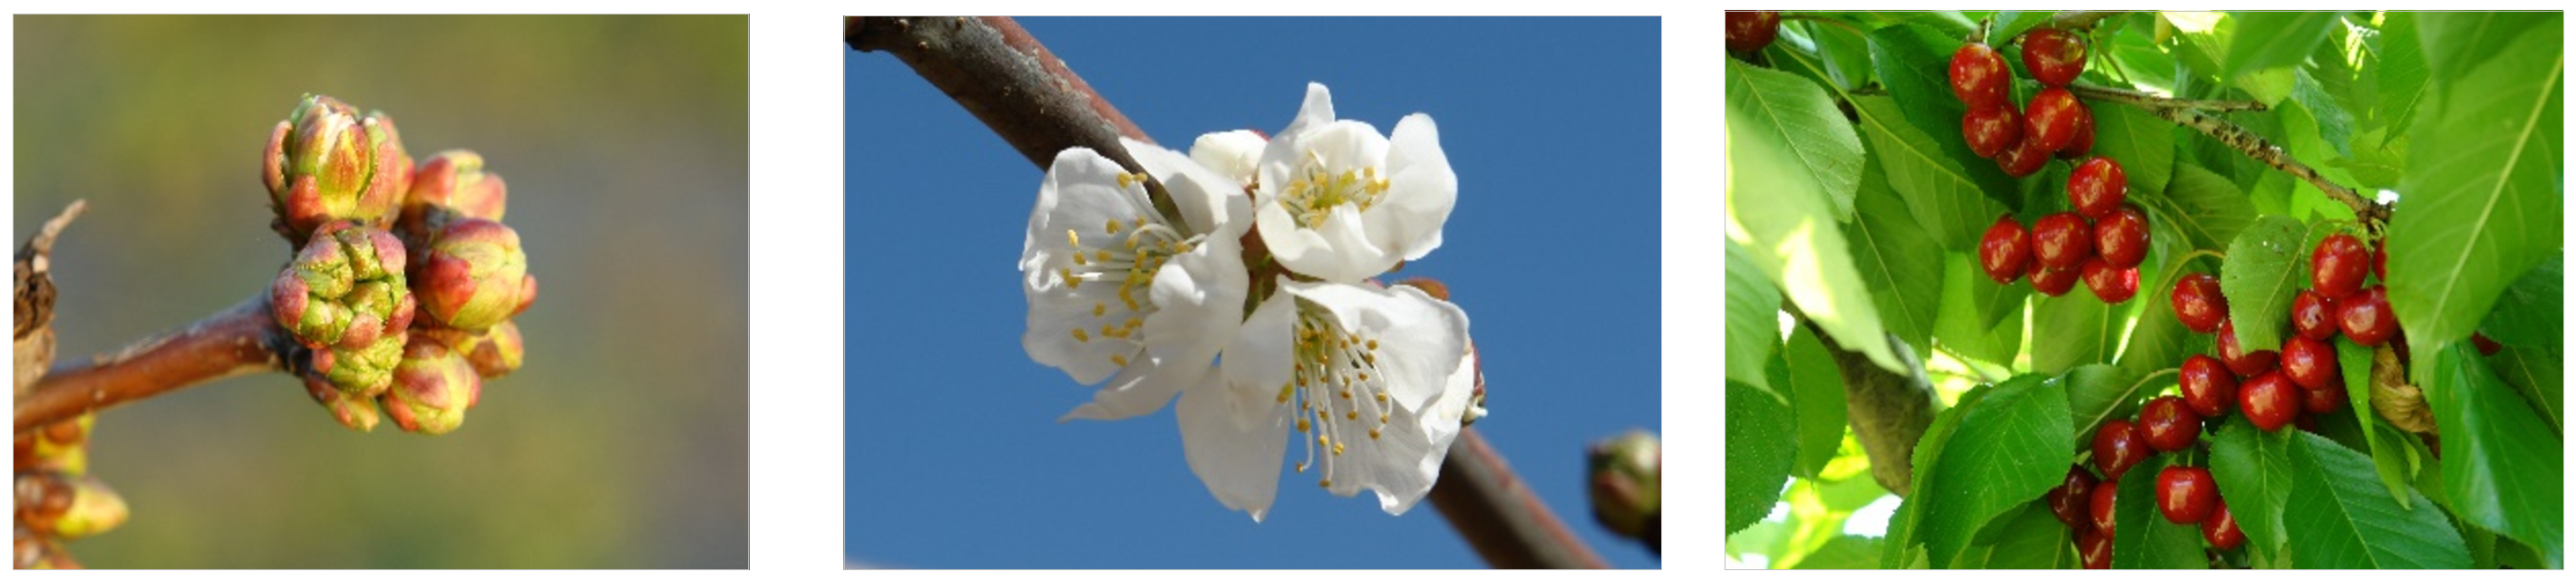
\includegraphics{./pheno_stages.png}
\caption{Picture 1 BBCH =55; Picture 2 BBCH =67; Picture 3 BBCH =89}
\end{figure}

\hypertarget{climate-change-and-impact-projection}{%
\chapter{Climate change and impact projection}\label{climate-change-and-impact-projection}}

\hypertarget{task-1-1}{%
\section{Task 1}\label{task-1-1}}

\textbf{List the main drivers of climate change at the decade to century scale, and briefly explain the mechanism through which the currently most important driver affects our climate}

\begin{table}

\caption{\label{tab:unnamed-chunk-2}Drivers of Climate Change}
\centering
\begin{tabular}[t]{l}
\hline
Drivers of climate change\\
\hline
Sun\\
\hline
Aerosols\\
\hline
Clouds\\
\hline
Ozone\\
\hline
Surface albedo\\
\hline
Greenhouse gases\\
\hline
\end{tabular}
\end{table}

\begin{quote}
The most important factor that currently has the greatest influence on climate and climate change is greenhouse gases. The most important greenhouse gases are water vapor, (carbon dioxide) CO2, (methane) CH4, and (nitrous oxides) N2O. Greenhouse gases can only absorb radiation of certain wavelengths. They absorb radiation with long wavelengths, which comes from the Earth's surface in the form of infrared radiation emitted by the warm Earth's surface. This radiation cannot leave the atmosphere and is trapped by the greenhouse gases, which returns it back to the Earth.
\end{quote}

\hypertarget{task-2-1}{%
\section{Task 2}\label{task-2-1}}

\textbf{Explain briefly what is special about temperature dynamics of the recent decades, and why we have good reasons to be concerned}

\begin{quote}
Over the past decades and throughout the last century, the temperature has been rising worldwide. Initially, this increase was relatively slow. The ten warmest years worldwide since 1880 were all measured after the millennium. The five warmest years worldwide were all recorded after 2014. This effect is also noticeable in Germany. Here, too, the ten warmest years were all measured after 2000, with one exception. If one places the temperature increase of the last decades in the climate history of the last one million years, it can be seen that there has never been such a strong temperature increase over such a relatively short period of time.

This rapid rise in temperature is developing its own dynamic. For example, high temperatures in the tundra cause the permafrost to thaw, releasing a large amount of CO2, a greenhouse gas that promotes even faster warming.
\end{quote}

\hypertarget{manual-chill-analysis}{%
\chapter{Manual Chill Analysis}\label{manual-chill-analysis}}

\begin{quote}
The \texttt{Winters\_hours\_gaps} data set has the columns: \texttt{Year}, \texttt{Month}, \texttt{Day}, \texttt{Hour}, \texttt{Temp\_gaps}, \texttt{Temp}. First, the function \texttt{cleaned\_data} is used to remove unnecessary columns such as \texttt{Temp\_gaps()} from the data set.
\end{quote}

\begin{Shaded}
\begin{Highlighting}[]
\CommentTok{#Clean Function}
\NormalTok{cleaned_data =}\StringTok{ }\ControlFlowTok{function}\NormalTok{(data_source) \{}
\NormalTok{  data_source =}\StringTok{ }
\StringTok{    }\NormalTok{data_source[, }\KeywordTok{c}\NormalTok{(}\StringTok{"Year"}\NormalTok{, }\StringTok{"Month"}\NormalTok{, }\StringTok{"Day"}\NormalTok{, }\StringTok{"Hour"}\NormalTok{, }\StringTok{"Temp"}\NormalTok{)]}
  \KeywordTok{return}\NormalTok{(data_source)}
\NormalTok{\}}

\CommentTok{# Apply Function to Winters_hours_gaps}
\KeywordTok{kable}\NormalTok{(}\KeywordTok{head}\NormalTok{(}\KeywordTok{cleaned_data}\NormalTok{(}\DataTypeTok{data_source =}\NormalTok{ Winters_hours_gaps)), }
      \StringTok{"pipe"}\NormalTok{, }\DataTypeTok{caption =} \StringTok{"Cleaned  Dataset: Winters_hours_gaps"}\NormalTok{)}
\end{Highlighting}
\end{Shaded}

\begin{longtable}[]{@{}rrrrr@{}}
\caption{\label{tab:unnamed-chunk-4}Cleaned Dataset: Winters\_hours\_gaps}\tabularnewline
\toprule
Year & Month & Day & Hour & Temp\tabularnewline
\midrule
\endfirsthead
\toprule
Year & Month & Day & Hour & Temp\tabularnewline
\midrule
\endhead
2008 & 3 & 3 & 10 & 15.127\tabularnewline
2008 & 3 & 3 & 11 & 17.153\tabularnewline
2008 & 3 & 3 & 12 & 18.699\tabularnewline
2008 & 3 & 3 & 13 & 18.699\tabularnewline
2008 & 3 & 3 & 14 & 18.842\tabularnewline
2008 & 3 & 3 & 15 & 19.508\tabularnewline
\bottomrule
\end{longtable}

\hypertarget{task-1-2}{%
\section{Task 1}\label{task-1-2}}

\textbf{Write a basic function that calculates warm hours (\textgreater25°C)}

\begin{Shaded}
\begin{Highlighting}[]
\NormalTok{WH <-}\StringTok{ }\ControlFlowTok{function}\NormalTok{(hourtemps)}
\NormalTok{\{}
\NormalTok{  hourtemps[, }\StringTok{"warm_hours"}\NormalTok{] <-}\StringTok{ }\NormalTok{hourtemps}\OperatorTok{$}\NormalTok{Temp }\OperatorTok{>=}\StringTok{ }\FloatTok{25.0}
  \KeywordTok{return}\NormalTok{(hourtemps)}
\NormalTok{\}}
\end{Highlighting}
\end{Shaded}

\hypertarget{task-2-2}{%
\section{Task 2}\label{task-2-2}}

\textbf{Apply this function to the Winters\_hours\_gaps dataset}

\begin{Shaded}
\begin{Highlighting}[]
\CommentTok{# have a look to the data set}
\KeywordTok{kable}\NormalTok{(}\KeywordTok{head}\NormalTok{(Winters_hours_gaps), }
      \StringTok{"pipe"}\NormalTok{, }\DataTypeTok{caption =} 
        \StringTok{"Example Dataset: Winters_hours_gaps"}\NormalTok{) }
\end{Highlighting}
\end{Shaded}

\begin{longtable}[]{@{}rrrrrr@{}}
\caption{\label{tab:unnamed-chunk-6}Example Dataset: Winters\_hours\_gaps}\tabularnewline
\toprule
Year & Month & Day & Hour & Temp\_gaps & Temp\tabularnewline
\midrule
\endfirsthead
\toprule
Year & Month & Day & Hour & Temp\_gaps & Temp\tabularnewline
\midrule
\endhead
2008 & 3 & 3 & 10 & 15.127 & 15.127\tabularnewline
2008 & 3 & 3 & 11 & 17.153 & 17.153\tabularnewline
2008 & 3 & 3 & 12 & 18.699 & 18.699\tabularnewline
2008 & 3 & 3 & 13 & 18.699 & 18.699\tabularnewline
2008 & 3 & 3 & 14 & 18.842 & 18.842\tabularnewline
2008 & 3 & 3 & 15 & 19.508 & 19.508\tabularnewline
\bottomrule
\end{longtable}

\begin{Shaded}
\begin{Highlighting}[]
\CommentTok{# Apply Function}
\NormalTok{hourtemps =}\StringTok{ }\KeywordTok{cleaned_data}\NormalTok{(}\DataTypeTok{data_source =}\NormalTok{ Winters_hours_gaps)}
\KeywordTok{kable}\NormalTok{(}\KeywordTok{head}\NormalTok{(}\KeywordTok{WH}\NormalTok{(}\DataTypeTok{hourtemps =}\NormalTok{ hourtemps)), }\StringTok{"pipe"}\NormalTok{)}
\end{Highlighting}
\end{Shaded}

\begin{longtable}[]{@{}rrrrrl@{}}
\toprule
Year & Month & Day & Hour & Temp & warm\_hours\tabularnewline
\midrule
\endhead
2008 & 3 & 3 & 10 & 15.127 & FALSE\tabularnewline
2008 & 3 & 3 & 11 & 17.153 & FALSE\tabularnewline
2008 & 3 & 3 & 12 & 18.699 & FALSE\tabularnewline
2008 & 3 & 3 & 13 & 18.699 & FALSE\tabularnewline
2008 & 3 & 3 & 14 & 18.842 & FALSE\tabularnewline
2008 & 3 & 3 & 15 & 19.508 & FALSE\tabularnewline
\bottomrule
\end{longtable}

\hypertarget{task-3-1}{%
\section{Task 3}\label{task-3-1}}

\textbf{Extend this function, so that it can take start and end dates as inputs and sums up warm hours between these dates}

\begin{Shaded}
\begin{Highlighting}[]
\NormalTok{warm_hours_function =}\StringTok{ }\ControlFlowTok{function}\NormalTok{(Input_Data,}
\NormalTok{                               S_Jahr,}
\NormalTok{                               S_Monat,}
\NormalTok{                               S_Tag,}
\NormalTok{                               S_Stunde,}
\NormalTok{                               E_Jahr,}
\NormalTok{                               E_Monat,}
\NormalTok{                               E_Tag,}
\NormalTok{                               E_Stunde) \{}
\NormalTok{  Start_Date <-}
\StringTok{    }\KeywordTok{which}\NormalTok{(}
\NormalTok{      hourtemps}\OperatorTok{$}\NormalTok{Year }\OperatorTok{==}\StringTok{ }\NormalTok{S_Jahr }\OperatorTok{&}\StringTok{ }\NormalTok{hourtemps}\OperatorTok{$}\NormalTok{Month }\OperatorTok{==}\StringTok{ }\NormalTok{S_Monat }\OperatorTok{&}
\StringTok{        }\NormalTok{hourtemps}\OperatorTok{$}\NormalTok{Day }\OperatorTok{==}\StringTok{ }\NormalTok{S_Tag }\OperatorTok{&}
\StringTok{        }\NormalTok{hourtemps}\OperatorTok{$}\NormalTok{Hour }\OperatorTok{==}\StringTok{ }\NormalTok{S_Stunde}
\NormalTok{    )}
\NormalTok{  End_Date <-}\StringTok{ }\KeywordTok{which}\NormalTok{(}
\NormalTok{    hourtemps}\OperatorTok{$}\NormalTok{Year }\OperatorTok{==}\StringTok{ }\NormalTok{E_Jahr }\OperatorTok{&}\StringTok{ }\NormalTok{hourtemps}\OperatorTok{$}\NormalTok{Month }\OperatorTok{==}\StringTok{ }\NormalTok{E_Monat }\OperatorTok{&}
\StringTok{      }\NormalTok{hourtemps}\OperatorTok{$}\NormalTok{Day }\OperatorTok{==}\StringTok{ }\NormalTok{E_Tag }\OperatorTok{&}\StringTok{ }\NormalTok{hourtemps}\OperatorTok{$}\NormalTok{Hour }\OperatorTok{==}\StringTok{ }\NormalTok{E_Stunde}
\NormalTok{  )}
  
  \CommentTok{# Apply Function Warm Hours (WH)}
\NormalTok{  hourtemps =}\StringTok{ }\KeywordTok{WH}\NormalTok{(}\DataTypeTok{hourtemps =}\NormalTok{ Input_Data)}
  
  \CommentTok{# Calculate warm_hours}
\NormalTok{  warm_hours =}\StringTok{ }\KeywordTok{sum}\NormalTok{(hourtemps}\OperatorTok{$}\NormalTok{warm_hours[Start_Date}\OperatorTok{:}\NormalTok{End_Date])}
  
  \KeywordTok{return}\NormalTok{(}\KeywordTok{cat}\NormalTok{(}\StringTok{"The number of heat hours is:"}\NormalTok{, }\KeywordTok{paste}\NormalTok{(warm_hours)))}
\NormalTok{\}}

\KeywordTok{warm_hours_function}\NormalTok{(}
  \DataTypeTok{Input_Data =}\NormalTok{ hourtemps,}
  \DataTypeTok{S_Jahr =} \DecValTok{2008}\NormalTok{,}
  \DataTypeTok{S_Monat =} \DecValTok{5}\NormalTok{,}
  \DataTypeTok{S_Tag =} \DecValTok{1}\NormalTok{,}
  \DataTypeTok{S_Stunde =} \DecValTok{12}\NormalTok{,}
  \DataTypeTok{E_Jahr =} \DecValTok{2008}\NormalTok{,}
  \DataTypeTok{E_Monat =} \DecValTok{8}\NormalTok{,}
  \DataTypeTok{E_Tag =} \DecValTok{31}\NormalTok{,}
  \DataTypeTok{E_Stunde =} \DecValTok{12}
\NormalTok{)}
\end{Highlighting}
\end{Shaded}

\begin{verbatim}
## The number of heat hours is: 957
\end{verbatim}

  \bibliography{book.bib,packages.bib}

\end{document}
